\documentclass[landscape,a2,final,12pt]{issposter}

\usepackage[latin1]{inputenc}
\usepackage{multicol}
\usepackage{graphicx,wrapfig}
\usepackage[english]{babel}
\usepackage{amsmath}
\usepackage{amsfonts}
\usepackage{amssymb}
\usepackage{dsfont}
\usepackage{caption}
\usepackage[font=scriptsize,labelfont=bf]{caption}
%\usepackage{enumitem} \setlist[itemize]{noitemsep}
\usepackage{enumitem}

\setlength{\abovecaptionskip}{5pt plus 3pt minus 2pt} % distance between image and caption

\renewcommand{\titlesize}{\LARGE}
\renewcommand{\sectionsize} {\Large}
\renewcommand{\authorsize}{\Large}
\renewcommand{\instsize}{\large}

\title{\MakeUppercase{Great Barrier Reef: Invasive Starfish Detector}}
\author{Nick Wagner and David Unger}
\institute{Institute of Signal Processing and System Theory, University of Stuttgart, Germany}
\conference{\normalsize \textbf{Deep Learning Lab 2022}, February 8, Stuttgart, Germany }

\begin{document}
\begin{samepage}
\maketitle

% Justified text sometimes looks strange in narrow columns
\raggedright
\begin{multicols}{3}

%%%%%%%%%%%%%%%%%%%%%%%%%%%%%%%%%%%%%%%%%%%%%%%%
\section{Problem Statement}
    \textbf{Abstract}\\
    \begin{small} The Great Barrier Reef in Australia is known world-wide for its diverse animal and coral species.
        Recently, the overpopulation of the coral-eating crown-of-thorns starfish starts threatening the existance of many corals.
        To allow divers to efficiently remove these star fishes from the corals, an object detection algorithm gets used. \newline
        The algorithm is based on the ''YOLO''--framework and takes video sequences as input, detects the starfishes and draws bounding boxes around them.\\
    \end{small}
    \vspace{0.5cm}
    \textbf{Dataset}
    %starfish image 
    \begin{wrapfigure}{r}{0pt}
    \centering
        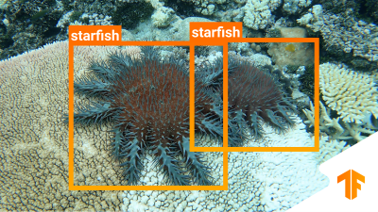
\includegraphics[scale=0.8]{1_starfishes.png}
        \caption{Example bounding boxes [1]}
    \end{wrapfigure} 
    \vspace*{-0.5cm}
    \begin{small}
    \begin{itemize}
        \item \raisebox{-0.6ex}{\~{}}23000 images\\ from 3 video sequences
        \item bounding box labels from csv
        \item binary problem
    \end{itemize}
    \end{small}
    \vspace*{2cm}
    \columnbreak
%%%%%%%%%%%%%%%%%%%%%%%%%%%%%%%%%%%%%%%%%%%%%%%%
\section{Architecture}
    \begin{small}
        The basis for the following customized architecture is the YOLO ("You Only Look Once") paper.
        The most significant changes are the removal of a dense layer, the addition of a dropout layer and dimension changes.
    \end{small}

    \begin{center}
        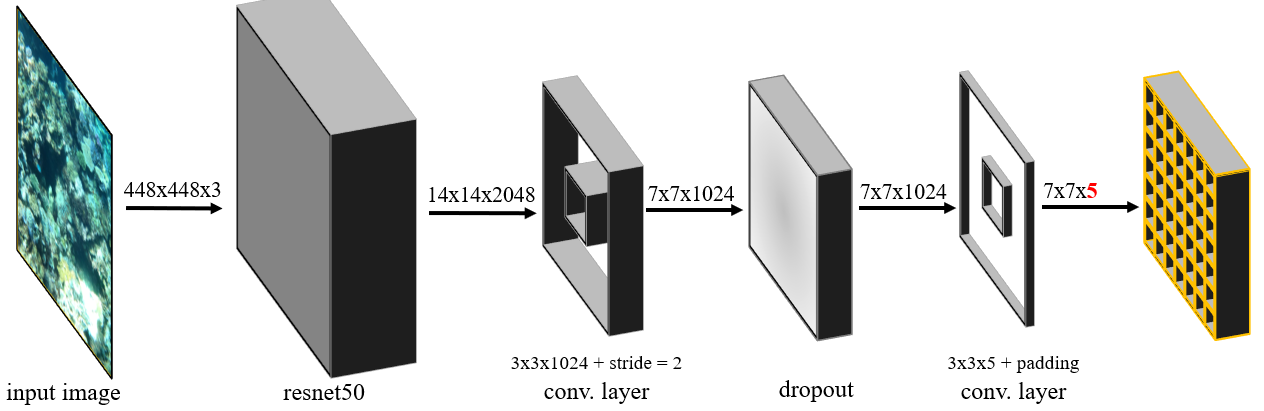
\includegraphics[scale=0.7]{2_architecture.png}
        \captionof{figure}{customized YOLO architecture}
    \end{center}
    \begin{small}
        \begin{itemize}
            \item {\textbf{input layer}: image size of 448x448 with three color channels (R,G,B)}
            \item {\textbf{resnet50}: transfer model that is pretrained on ImageNet data}
            \item {\textbf{conv1}: reduction of channels and grid size to 7x7 due to stride}
            \item {\textbf{dropout}: generalization technique to prevent overfitting}
            \item {\textbf{conv2}: final reduction of channels to 5 with padding}
        \end{itemize}
    \end{small}
    \columnbreak
%%%%%%%%%%%%%%%%%%%%%%%%%%%%%%%%%%%%%%%%%%%%%%%%    
\section{Network Output}
    \begin{small}
        The final output of the network is a 7x7 grid. Each grid cell predicts one bounding box, which results in 49 possibly predicted bounding boxes.
    \end{small}
    \begin{center}
        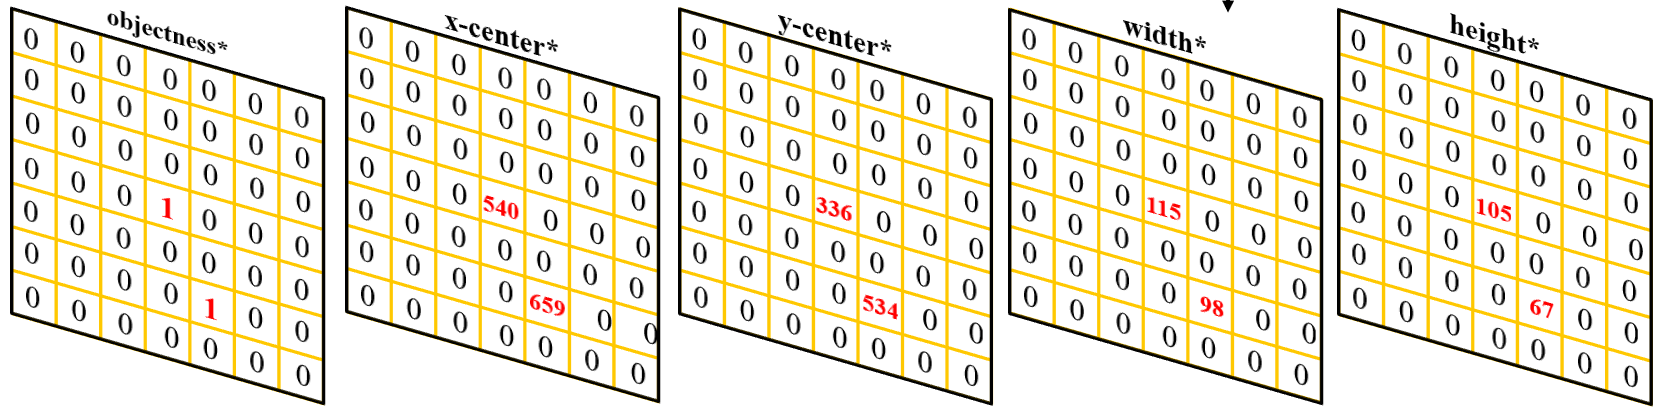
\includegraphics[scale=0.55]{3_channels.png}
        \captionof{figure}{customized YOLO architecture}
    \end{center}
    \begin{small}
        \begin{itemize}
            \item {\textbf{objectness}: confidence of the prediction}
            \item {\textbf{x-center}: x-coordinate in relation to its cell center}
            \item {\textbf{y-center}: y-coordinate in relation to its cell center}
            \item {\textbf{width}: box-width measured in cell widths}
            \item {\textbf{height}: box-height measured in cell heights}
        \end{itemize}
    \end{small}
    \begin{footnotesize}
        * The values are shown in pixel for understanding purposes. In reality, smaller values relative to the cell size are easier for the model to predict. Hence, the implementation is done that way.
    \end{footnotesize}
    
\end{multicols}


\rule{\textwidth}{8pt}

\begin{multicols}{3}
%%%%%%%%%%%%%%%%%%%%%%%%%%%%%%%%%%%%%%%%%%%%%%%%
\section{Input Pipeline}
        \begin{small}Compared to a classification network, a detection network requires a more complicated input pipeline. This mainly comes from the 
        labels which are dependent on the image content and scale, rotation, crop and flip variant.Therefore, the input pipeline consists of the following steps:
        \begin{itemize}
            \item CSV loading
            \item Bounding box text to grid conversion
            \item Image reading and resizing
            \item Image augmentation
        \end{itemize}

        \begin{center}
            \includegraphics[scale=0.05]{4_augmentation.png}
            \captionof{figure}{input image augmentated differently }
        \end{center}

        \end{small}
       
    \columnbreak
%%%%%%%%%%%%%%%%%%%%%%%%%%%%%%%%%%%%%%%%%%%%%%%%
    \section{Loss Function}
        \begin{minipage}[b]{0.3\textwidth}
            \begin{scriptsize} To ensure that the network learns the bounding boxes as represented by the ground truth labels, 
            using a standard loss function is not sufficient. Therefore, the loss function from the YOLO paper is used and adapted 
            that it fits the described problem setup.
            
            The four parts of our loss function are the following and summed up during training 
            \begin{itemize}
                \item Objectness loss: \quad $l_{obj} = \lambda_{obj} \sum_{i=0}^{(S-1)^2} \mathds{1}_{i}^{obj} (1 - \hat{p}_i)^2  $
                \item No object loss: \quad \quad $l_{noobj} = \lambda_{noobj} \sum_{i=0}^{(S-1)^2} \mathds{1}_{i}^{noobj} (0 - \hat{p}_i)^2  $
                \item BBox center loss: \quad $l_{center} = \lambda_{center} \sum_{i=0}^{(S-1)^2} \mathds{1}_{i}^{obj} [(x_i - \hat{x}_i)^2 + (y_i - \hat{y}_i)^2] $
                \item BBox size loss: \quad \quad$l_{size} = \lambda_{size} \sum_{i=0}^{(S-1)^2} \mathds{1}_{i}^{obj} [(\sqrt{w_i} - \sqrt{\hat{w}_i})^2 + (\sqrt{h_i} - \sqrt{\hat{h}_i})^2] $
            \end{itemize}

            The loss term weightings $\lambda$ are determined in a way, that all loss terms are in a 
            similar range and therefore are optimized in a similar strength.

            \begin{figure}
                \centering
                \begin{minipage}{.5\textwidth}
                \centering
                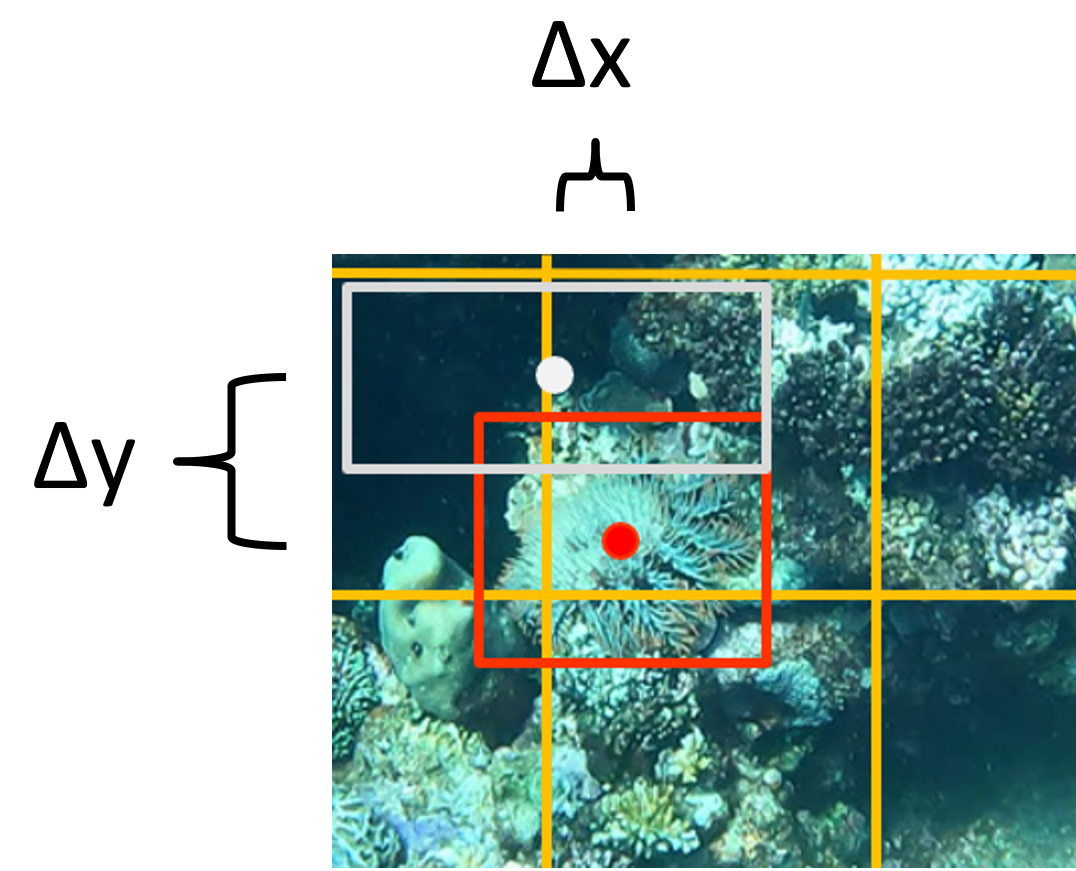
\includegraphics[width=.4\linewidth]{5_loss_center.png}
                \captionof{figure}{A figure}
                \label{fig:test1}
                \end{minipage}%
                \begin{minipage}{.5\textwidth}
                \centering
                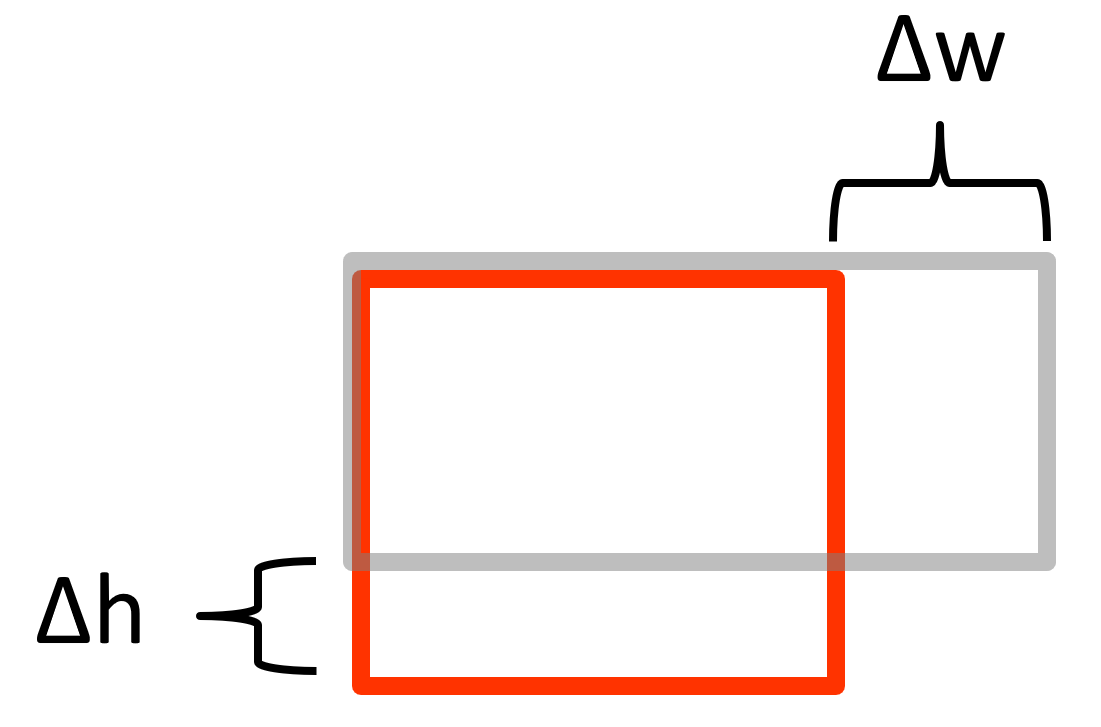
\includegraphics[width=.4\linewidth]{5_loss_size.png}
                \captionof{figure}{Another figure}
                \label{fig:test2}
                \end{minipage}
                \end{figure}
            

            \end{scriptsize}
        \end{minipage}

    \columnbreak
%%%%%%%%%%%%%%%%%%%%%%%%%%%%%%%%%%%%%%%%%%%%%%%%    
    \section{Challenge}
        \begin{minipage}[b]{0.3\textwidth}
            \begin{scriptsize}Compared to a classification network, a detection network requires a more complicated input pipeline. This mainly comes from the 
                labels which are dependent on the image content and scale, rotation, crop and flip variant.Therefore, the input pipeline consists of the following steps:
                \begin{itemize}
                    \item CSV loading
                    \item Bounding box text to grid conversion
                    \item Image reading and resizing
                    \item Image augmentation
                \end{itemize}

                \begin{center}
                    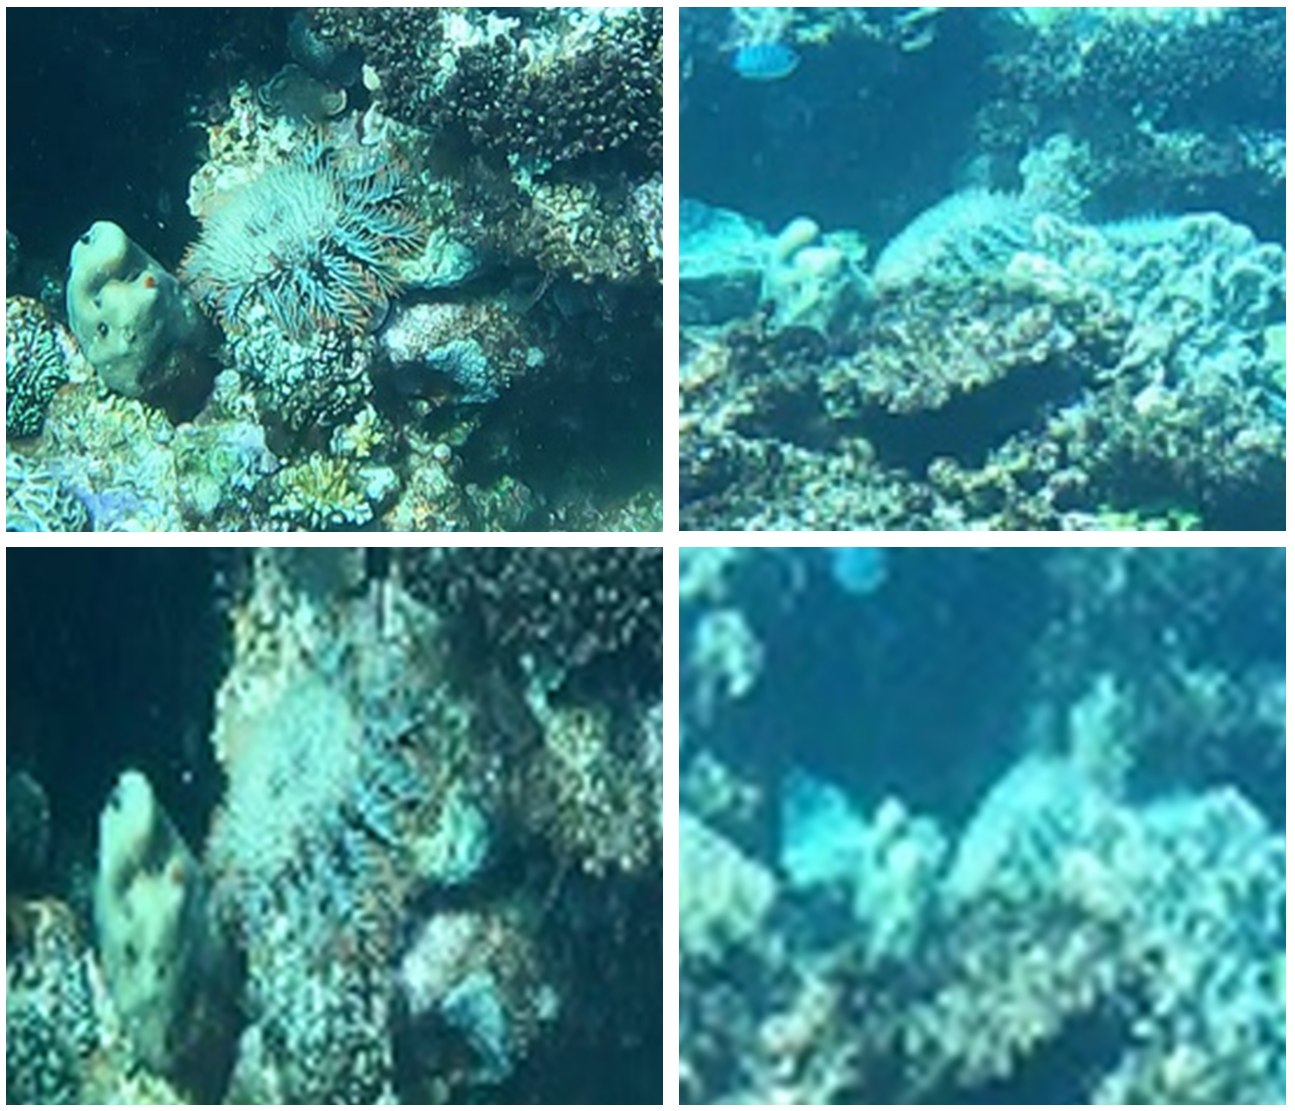
\includegraphics[scale=0.3]{6_img_quality.png}
                    \captionof{figure}{Starfish at downscaled images with poor quality}
                \end{center}

            \end{scriptsize}
        \end{minipage}
    \columnbreak
\end{multicols}
\end{samepage}
\end{document}


